\documentclass{beamer}

\usepackage[utf8]{inputenc}
\usepackage[english]{babel}
\usepackage{amsmath}
\usepackage{amssymb}
\usepackage{amsthm}
\usepackage{commath}
\usepackage{mathtools}
\usepackage{faktor}
\usepackage{color}
\usepackage{graphicx}
\usepackage{multirow}
\usepackage{array}
\usepackage{multirow}
\usepackage{breqn}
\usepackage[adversary, operators, sets, primitives, notions, probability, advantage, ff]{cryptocode}
\usepackage{todonotes}
\usepackage{tikz-cd}
\usepackage{hyperref}



%\addtolength{\topmargin}{-.5in}
%\addtolength{\textheight}{0.5in}
\allowdisplaybreaks



\newcommand{\manuela}[1]{\todo[inline, color=lime]{{ Manuela:} #1}}


\newcommand{\zdv}{\adversary{Z}}
\newcommand{\Fun}{\mathcal{F}}
\newcommand{\keygen}{\mathsf{KeyGen}}
\newcommand{\encaps}{\mathsf{Encaps}}
\newcommand{\decaps}{\mathsf{Decaps}}


\DeclareMathOperator{\lcm}{lcm}
\DeclareMathOperator{\Imm}{Im}
\DeclareMathOperator{\Dom}{Dom}
\DeclareMathOperator{\End}{End}
\DeclareMathOperator{\Hom}{Hom}
\DeclareMathOperator{\Aut}{Aut}
\DeclareMathOperator{\car}{char}
\DeclareMathOperator{\st}{\; |\;}
\DeclareMathOperator{\et}{\;\wedge\;}
\DeclareMathOperator{\tr}{Tr}
\DeclareMathOperator{\n}{N}
\DeclareMathOperator{\disc}{disc}
\DeclareMathOperator{\GL}{GL}


\newcommand{\N}{\mathbb{N}}
\newcommand{\Z}{\mathbb{Z}}
\newcommand{\Q}{\mathbb{Q}}
\newcommand{\R}{\mathbb{R}}
\newcommand{\C}{\mathbb{C}}
\newcommand{\F}{\mathbb{F}}
\newcommand{\Oc}{\mathcal{O}}
\newcommand{\Zn}[1]{\Z/#1\Z}
\newcommand{\ds}{\displaystyle}
\newcommand{\eps}{\varepsilon}



\usetheme{Frankfurt}
\useinnertheme{circles}
%\useoutertheme{miniframes}


\title{Isogeny-based Oblivious Transfer Protocols}
\author{Riccardo Zanotto}
\date{December 17, 2021}


\begin{document}
    
    \createprocedureblock{myproc}{center, boxed}{}{}{}
    
    \begin{frame}
        \maketitle
    \end{frame}

    \begin{frame}
        \frametitle{Contents}
        \tableofcontents
    \end{frame}

    \section{Oblivious transfer}
    \begin{frame}
        \frametitle{What is oblivious transfer?}
        
        \begin{center}
        \begin{bbrenv}{A}
            
            \begin{bbrbox}[name=OT, namepos=middle, minheight=2cm]
                
            \end{bbrbox}
            \bbrmsgto{top={$(m_0,m_1)$},fixedoffset=2ex,length=1.5cm}
            \bbrmsgtxt[xshift=1.5cm]{\includegraphics[height=5cm]{images/Alice}}
            
            \bbrqryfrom{top=$\sigma$,fixedoffset=2ex,length=1.5cm}
            \bbrqryto{top=$m_\sigma$,fixedboffset=2ex,length=1.5cm}
            \bbrqrytxt[]{\includegraphics[height=5cm]{images/Bob}}
            
        \end{bbrenv}
        \end{center}        
    \end{frame}

    \begin{frame}
        \frametitle{Multi-party computation}
        
        \centering
        \includegraphics[width=0.9\textwidth]{images/MPC}
    \end{frame}

    \begin{frame}
        \frametitle{Why?}
        \begin{block}{Why MPC?}
            MPC studies the task of \emph{computing on private data}; sillier and serious examples:
            \begin{itemize}
                \item Deciding who is richer between two people without revealing their total worth.
                \item Running auctions with secret bidding.
                \item Distributed voting.
                \item Threshold signatures or decryptions.
                \item Running machine learning models on sensitive information, like X-ray pictures.
            \end{itemize}
        \end{block}
    

    \end{frame}

    \begin{frame}
        \frametitle{Why?}
        \begin{block}{Why OT?}
            Oblivious transfer is defined by a very simple function: $$f((m_0,m_1),\sigma)=(\lambda,m_\sigma)$$
            It can be used as a \emph{building block} of any MPC protocol, via the GMW construction (or \emph{garbled circuits}).
        \end{block}
    
        \pause
        \begin{block}{What do we want from OT?}
            \begin{itemize}
                \item Efficiency: for MPC we require many OTs; ususally they use public key cryptography (slow), so we need to keep low the number of rounds and the public key operations.
                \item Security: since the OTs can be run in parallel, we want privacy for concurrent executions and compositions.
            \end{itemize}
        \end{block}
    
    \end{frame}

    \begin{frame}
        \frametitle{The simplest OT by Chou and Orlandi}
        
        \begin{block}{The protocol}
                    \begin{center}
                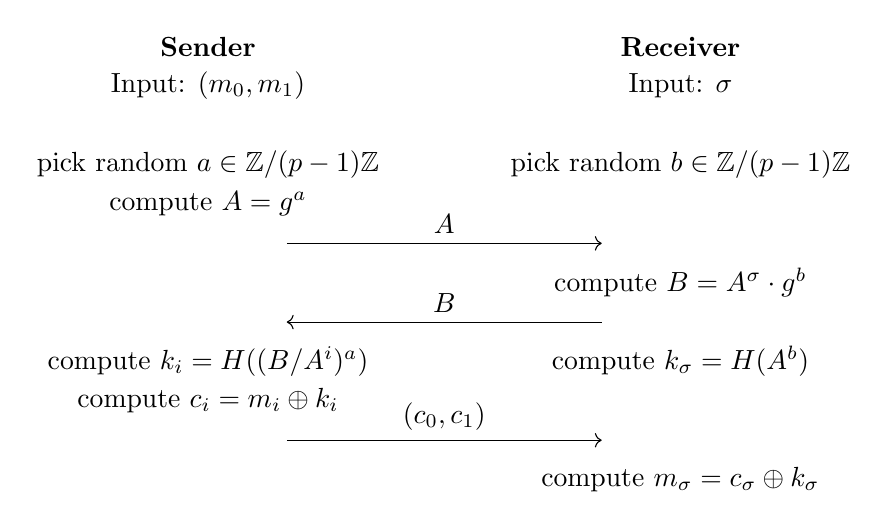
\begin{tikzpicture}
                \node at (0,0) {\bf Sender};
                \node at (6,0) {\bf Receiver};
                \node at (0,-0.5) {Input: $(m_0,m_1)$};
                \node at (6,-0.5) {Input: $\sigma$};
                \node at (0,-1.5) {pick random $a\in\Zn{(p-1)}$};
                \node at (0,-2) {compute $A=g^a$};
                \node at (6,-1.5) {pick random $b\in\Zn{(p-1)}$};          
                \draw[->] (1,-2.5) to node[auto] {$A$} (5,-2.5);
                \node at (6,-3) {compute $B=A^\sigma\cdot g^b$};
                \draw[->] (5,-3.5) to node[above] {$B$} (1,-3.5);
                \node at (0,-4) {compute $k_i=H((B/A^i)^a)$};
                \node at (6,-4) {compute $k_\sigma=H(A^b)$};
                \node at (0,-4.5) {compute $c_i=m_i\oplus k_i$};
                \draw[->] (1,-5) to node[above] {$(c_0,c_1)$} (5,-5);
                \node at (6,-5.5) {compute $m_\sigma=c_\sigma\oplus k_\sigma$};
                \end{tikzpicture}
            \end{center}
        \end{block}
        

    \end{frame}

    \begin{frame}
        \frametitle{The problems of simplest OT}
        
        \begin{block}{Why not?}
            \begin{itemize}[<+->]
                \item Uses Diffie-Hellman: Shor's quantum algorithm solves the discrete logarithm problem in polynomial time. If we want security in a world with quantum computers, we need new cryptography.
                \item Wrong security proof: the proofs for MPC protocols are done in the Universal Composability framework and require many details; other cryptographers noticed that the authors missed some of them. There seems to be no way of fixing the proof.
            \end{itemize}
        \end{block}
    \end{frame}


    \section{Isogeny-based cryptography}
    
    \begin{frame}
        \frametitle{Post-quantum cryptography}
        
        \begin{block}{The problem}
            In 1994 Shor found a quantum polynomial algorithm for \emph{order finding}. With this, it is possible to solve dicrete logarithms in any abelian group and to factor large integers.
            
            Most of public key cryptography is then broken (RSA, DH, ECDH).
        \end{block}
    
        \pause
        \begin{block}{The solution}
            In 2016 NIST started a competition to find new \emph{post-quantum} public key primitives. The proposals are based on:
            \begin{itemize}
                \item Lattices
                \item Codes
                \item Multivariate equation
                \item \color<3->{red}{Supersingular isogenies}
            \end{itemize}
        \end{block}
    \end{frame}

    \begin{frame}
        \frametitle{Elliptic curves}
        
        \begin{definition}
            An \emph{elliptic curve} $E$ \emph{over} $K$ is a smooth projective curve of genus $1$, with a given $K$-rational point.
        \end{definition}
    
        \begin{block}{For cryptographers}
            An elliptic curve $E$ is a Weierstrass equation $$y^2=x^3+ax+b$$ where $4a^3+27b^2\neq0$; don't forget the point at infinity!
        \end{block}
    
        \begin{theorem}
            Let $E$ be an elliptic curve over $K$; then $E(K)$ has an abelian group structure $\oplus$, with neutral element the point at infinity.
        \end{theorem}
    \end{frame}

    \begin{frame}
        \frametitle{The group law}
        \begin{center}
            \begin{tikzpicture}[domain=-2.4566:4,samples=100,yscale=1/2]
            \draw plot (\x,{sqrt(\x*\x*\x-4*\x+5)});
            \draw plot (\x,{-sqrt(\x*\x*\x-4*\x+5)});
            
            \draw[thin,gray,-latex] (0,-7) -- (0,7);
            \draw[thin,gray,-latex] (-3,0) -- (4,0);
            \draw (-3,1) -- (4,8/3+3);
            \begin{scope}[every node/.style={draw,circle,inner sep=1pt,fill},cm={1,2/3,0,0,(0,3)}]
            \node at (-2.287980,0) {};
            \node at (-0.535051,0) {};
            \node at (3.267475,0) {};
            \end{scope}
            \begin{scope}[every node/.style={yshift=0.3cm},cm={1,2/3,0,0,(0,3)}]
            \node at (-2.287980,0) {$P$};
            \node at (-0.535051,0) {$Q$};
            \node at (3.267475,0) {$R$};
            \end{scope}
            
            \draw[dashed] (3.267475,3.267475*2/3+3) -- (3.267475,-3.267475*2/3-3) 
            node[draw,circle,inner sep=1pt,fill] {}
            node[xshift=-0.1cm,anchor=east] {$P\oplus Q$};
            \end{tikzpicture}
        \end{center}
    \end{frame}

    \begin{frame}
        \frametitle{Isogenies}
        
        \begin{definition}
            Let $E_1$ and $E_2$ be elliptic curves, with points at infinity $O_1,O_2$. An \emph{isogeny} is a morphism of curves $\phi:E_1\to E_2$ such that $\phi(O_1)=O_2$.
        \end{definition}
    
        \begin{theorem}
            Let $\phi:E_1 \to E_2$ be a non-constant isogeny. Then $\phi$ induces a surjective group homomorphism $E_1(\bar K)\to E_2(\bar K)$ with finite kernel.
            
            Moreover, separable isogenies are in bijection with finite subgroups of $E_1$.
        \end{theorem}
    
        \begin{block}{Vélu's formula}
            Given a subgroup $G<E(K)$ of an elliptic curve defined over $K$, there is a formula that in time $O(\# G)$ computes the corresponding isogeny and the codomain curve.
        \end{block}
    \end{frame}

    \begin{frame}
        \frametitle{Elliptic curves over finite fields}
        
        \begin{definition}
            Let $E/\F_q$ be an elliptic curve; then its Frobenius endomorphism is the morphism $\pi: E\to E$ given by $$\pi(X:Y:Z)=(X^q:Y^q:Z^q)$$
        \end{definition}
    
        \begin{theorem}
            Let $E/\F_q$ be an elliptic curve and $\pi$ its Frobenius endomorphism. Then there exists $t\in\Z$ such that $$\pi^2-t\pi+q=0.$$
            
            Moreover, $\# E(\F_q) = q+1-t$ with $|t|\le2\sqrt q$.
        \end{theorem}
    \end{frame}

    \begin{frame}
        \frametitle{Supersingular elliptic curves}
        
        \begin{theorem}
            Let $E/K$ be an elliptic curve, with $\car K=p$. The following are equivalent:
            \begin{enumerate}
                \item $E[p^r]=\{O\}$ for some (all) $r\ge1$.
                \item The dual isogeny $\hat\pi$ is inseparable.
                \item The map $[p]:E\to E$ is purely inseparable and $j(E)\in\F_{p^2}$.
                \item $\End(E)$ is a maximal order in a quaternion algebra.
                \item $p\mid t$, the trace of Frobenius.
            \end{enumerate}
            If any of these properties hold, we say that $E$ is \emph{supersingular}; otherwise $E$ is said to be \emph{ordinary}.
        \end{theorem}
    \end{frame}

    \begin{frame}
        \frametitle{The CM action}
        
        \begin{definition}
            Let $\Oc$ be an order in an imaginary quadratic field $K$, and denote by $Ell_q(\Oc)$ the set of $\F_q$-isomorphism classes of elliptic curves with \emph{complex multiplication} by $\Oc$, i.e. with $\End_{\F_q}(E)=\Oc$.
        \end{definition}
        
        \begin{theorem}
            Let $\F_q$ be a finite field and $\Oc\subset\Q(\sqrt{-D})$ an order in a quadratic imaginary field. Assume $Ell_q(\Oc)$ is non empty; then there is a free and transitive action given by
            \begin{align*}
            Cl(\Oc)\times Ell_q(\Oc) & \to  Ell_q(\Oc)\\
            (\mathfrak{a}, E) & \mapsto  E/E[\mathfrak{a}]
            \end{align*}
        \end{theorem}
    
    \end{frame}

    \begin{frame}
        \frametitle{CM graphs}
        
        \begin{center}
            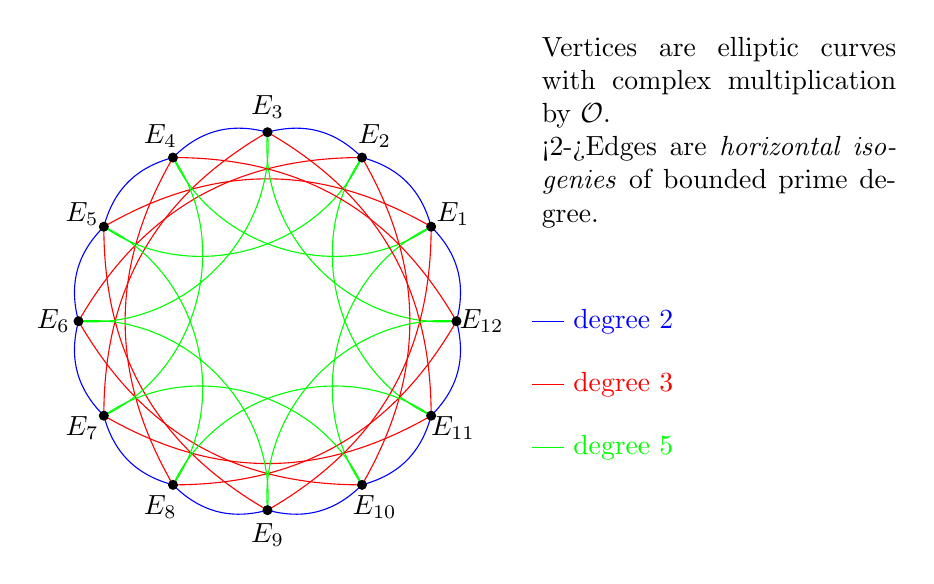
\begin{tikzpicture}[scale=0.8]
            \begin{scope}
            \def\crater{12}
            \def\jumpa{-8}
            \def\jumpb{9}
            \def\diam{3cm}
            
            \foreach \i in {1,...,\crater} {
                \uncover<2->{\draw[blue] (360/\crater*\i : \diam) to[bend right] (360/\crater*\i+360/\crater : \diam);}
                \uncover<3->{\draw[red] (360/\crater*\i : \diam) to[bend right] (360/\crater*\i+\jumpa*360/\crater : \diam);}
                \uncover<4->{\draw[green] (360/\crater*\i : \diam) to[bend right=50] (360/\crater*\i+\jumpb*360/\crater : \diam);}
            }
            \foreach \i in {1,...,\crater} {
                \draw[fill] (360/\crater*\i: \diam) circle (2pt) +(360/\crater*\i: 0.4) node{$E_{\i}$};
            }
            \end{scope}
            \begin{scope}[xshift=4.2cm]
            \draw (0,3) node[anchor=west] {\parbox{4.5cm}{%
                    Vertices are elliptic curves with complex
                        multiplication by $\Oc$.\\
                    \uncover<2->{Edges are \emph{horizontal isogenies} of
                        bounded prime degree.}  }};
            
            \uncover<2->{\draw[blue] (0,0) -- (0.5,0)
                (0.5,0) node[anchor=west] {degree $2$};}
            \uncover<3->{\draw[red] (0,-1) -- (0.5,-1) (0.5,-1)
                node[anchor=west] {degree $3$};}
            \uncover<4->{\draw[green]
                (0,-2) -- (0.5,-2) (0.5,-2) node[anchor=west] {degree $5$};}
            
            \end{scope}
            \end{tikzpicture}
        \end{center}
    
    \end{frame}

    \begin{frame}
        \frametitle{Diffie-Hellman}
        
        \begin{center}
            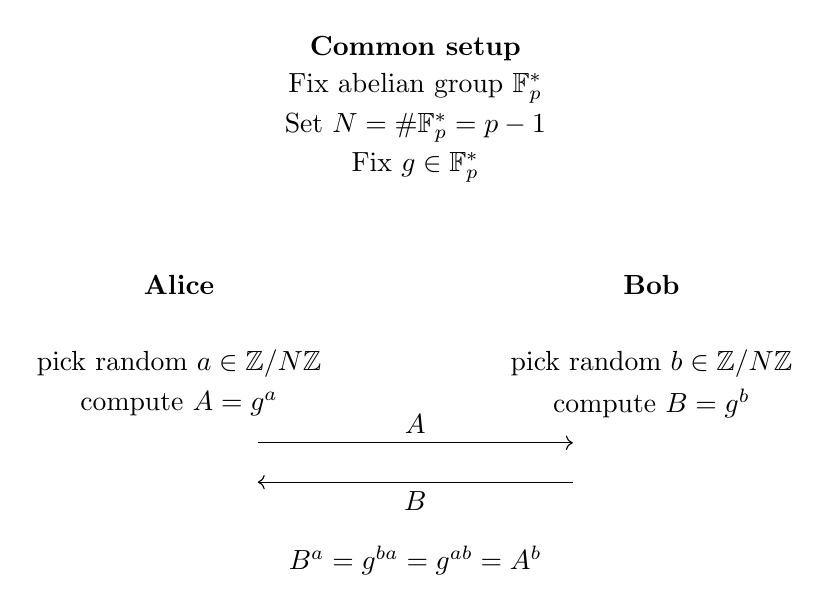
\begin{tikzpicture}
            \node at (3,3) {\bf Common setup};
            \node at (3,2.5) {Fix abelian group $\F_p^\ast$};
            \node at (3,2) {Set $N=\# \F_p^\ast=p-1$};
            \node at (3,1.5) {Fix $g\in\F_p^\ast$};
            \node at (0,0) {\bf Alice};
            \node at (6,0) {\bf Bob};
            \node at (0,-1) {pick random $a\in\Zn{N}$};
            \node at (0,-1.5) {compute $A=g^a$};
            \node at (6,-1) {pick random $b\in\Zn{N}$};
            \node at (6,-1.5) {compute $B=g^b$};
            \draw[->]
            (1,-2) to node[auto] {$A$} (5,-2);
            \draw[->] (5,-2.5) to node[auto] {$B$} (1,-2.5);
            \node at (3,-3.5) {\alert{$B^a=g^{ba}=g^{ab}=A^b$}};
            \end{tikzpicture}
        \end{center}
        
    \end{frame}

    \begin{frame}
    \frametitle{Hard homogeneous spaces}
    
    \begin{center}
        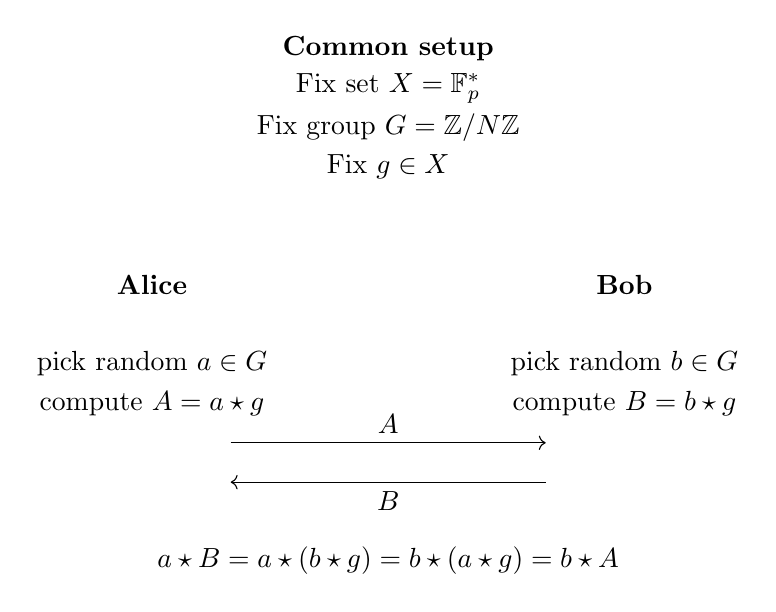
\begin{tikzpicture}
        \node at (3,3) {\bf Common setup};
        \node at (3,2.5) {Fix set $X=\F_p^\ast$};
        \node at (3,2) {Fix group $G=\Zn{N}$};
        \node at (3,1.5) {Fix $g\in X$};
        \node at (0,0) {\bf Alice};
        \node at (6,0) {\bf Bob};
        \node at (0,-1) {pick random $a\in G$};
        \node at (0,-1.5) {compute $A=a\star g$};
        \node at (6,-1) {pick random $b\in G$};
        \node at (6,-1.5) {compute $B=b\star g$};
        \draw[->]
        (1,-2) to node[auto] {$A$} (5,-2);
        \draw[->] (5,-2.5) to node[auto] {$B$} (1,-2.5);
        \node at (3,-3.5) {\alert{$a\star B= a\star(b\star g)=b\star(a\star g)=b\star A$}};
        \end{tikzpicture}
    \end{center}
    
    \end{frame}

    \begin{frame}
    \frametitle{A HHS from complex multiplication}
    
    \begin{center}
        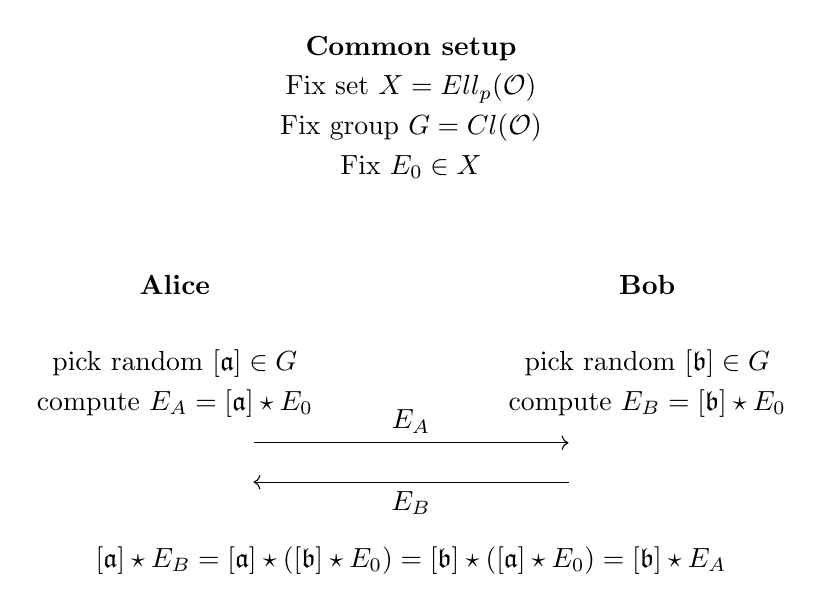
\begin{tikzpicture}
        \node at (3,3) {\bf Common setup};
        \node at (3,2.5) {Fix set $X=Ell_p(\Oc)$};
        \node at (3,2) {Fix group $G=Cl(\Oc)$};
        \node at (3,1.5) {Fix $E_0\in X$};
        \node at (0,0) {\bf Alice};
        \node at (6,0) {\bf Bob};
        \node at (0,-1) {pick random $[\mathfrak{a}]\in G$};
        \node at (0,-1.5) {compute $E_A=[\mathfrak{a}]\star E_0$};
        \node at (6,-1) {pick random $[\mathfrak{b}]\in G$};
        \node at (6,-1.5) {compute $E_B=[\mathfrak{b}]\star E_0$};
        \draw[->]
        (1,-2) to node[auto] {$E_A$} (5,-2);
        \draw[->] (5,-2.5) to node[auto] {$E_B$} (1,-2.5);
        \node at (3,-3.5) {\alert{$[\mathfrak{a}]\star E_B= [\mathfrak{a}]\star([\mathfrak{b}]\star E_0)=[\mathfrak{b}]\star([\mathfrak{a}]\star E_0)=[\mathfrak{b}]\star E_A$}};
        \end{tikzpicture}
    \end{center}
    
    \end{frame}


    \begin{frame}
        \frametitle{The CSIDH protocol}
        
        \begin{block}{The setting}
            Fix a prime prime of the form $p=4\ell_1\cdots\ell_n-1$; fix also $E_0:y^2=x^3+x$, which is supersingular over $\F_p$; define $\Oc:=\End_p(E_0)\cong\Z[\sqrt{-p}]$.
            
            \textbf{The group}: $Cl(\Oc)$.
            
            \textbf{The set}: $Ell_p(\Oc)$.
            
            \textbf{The action}: we only use particular ideals (and their inverses) $\mathfrak{l}_i=(\ell_i,\pi-1)$, which generate $Cl(\Oc)$. The action is easy to compute with Vélu's formula, since $E[\mathfrak{l}_i]=E[\ell_i]\cap E(\F_p)$ has $\ell_i$ points, all defined over $\F_p$.
        \end{block}
    
        \begin{block}{Hard problems}
            \textbf{Vectorization}: given two curves $E,E'$, find $[\mathfrak{a}]\in Cl(\Oc)$ with smooth norm such that $[\mathfrak{a}]\star E = E'$.       
        \end{block}
    
    \end{frame}

    \begin{frame}
        \frametitle{Quantum security of CSIDH}
        
        \begin{block}{Subexponential attack}
            \begin{itemize}
                \item CSIDH, and any hard homogeneous space, reduces to the \emph{hidden shift problem}.
                \item Kuperberg's and Regev's quantum algorithms solve HShP in $O(\exp(\sqrt{\log \# G}))$ for generic $G$.
                \item For CSIDH, $G=Cl(\Oc)=Cl(\Z[\sqrt{-p}])$ thus $\# G\approx\sqrt{p}$.
                \item Precise estimations still debated, \texttt{CSIDH-512} might have $2^{64}$-qbit security.
            \end{itemize}
        \end{block}
    
    \end{frame}
    
    
    \section{Security definitions}
    
    \begin{frame}
        \frametitle{Perfect secrecy}
        
        \begin{definition}
            The one-time pad is an encryption scheme whose encryption and decryption functions are
            $$ \enc(k,m)=k\oplus m\;\;\;\;\; \dec(k,c)=k\oplus c,$$
            where $\oplus$ denotes the bit-wise XOR of the bitstrings.
        \end{definition}
    
        \begin{definition}
            We say that an encryption scheme $(\kgen,\enc,\dec)$ is \emph{perfectly secure} if for any $m_0,m_1\in\mathcal M$ and all $c\in\mathcal C$ it holds that 
            $$\prob{\enc(k,m_0)=c} = \prob{\enc(k,m_1)=c}$$
        \end{definition}
    
    \end{frame}

    \begin{frame}
        \frametitle{Simulation-based security}
        
        \begin{block}{The main idea}
            There is an \emph{ideal world} in which the adversary interacts only with a trusted third party; the \emph{real world} instead runs the actual protocol.
            
            If any real world adversary can be \emph{simulated} in the ideal world, then the protocol is \emph{secure}.
        \end{block}
    
        \begin{definition}
            Let $f=(f_1,f_2)$ be a functionality. We say that protocol $\pi$ \emph{securely computes $f$ in the presence of semi-honest adversaries} if there exists two PPT algorithms $\sdv_1,\sdv_2$ such that
            $$ \{ (\sdv_i(w^i,f_i(x,y)), f(x,y) ) \}_{x,y} \cindist \{ (\texttt{view}_i^\pi(x,y), \texttt{output}^\pi(x,y)) \}_{x,y} $$
            for both $i=1,2$. (recall that $w^1=x,w^2=y$)
        \end{definition}
    \end{frame}

    \begin{frame}
        \frametitle{Malicious adversaries}
        
        \begin{alertblock}{The problem}
            If the adversary can behave any way he wants, he could also \emph{change} the inputs he uses, and the simulator doesn't have access to them.
            
            The simulator has then to \emph{extract} the input of the corrupted parties from the adversary.
        \end{alertblock}
    
        \pause
        \begin{block}{The ideal execution}
            Suppose $x,y$ are the original inputs, and $\sdv$ controls $P_i$.
            \begin{itemize}
                \item Honest party $P_j$ sends its input to the trusted party.
                \item Corrupted party $P_i$ sends anyting he wants.
                \item Trusted party receives $(x',y')$ and computes $f(x',y')$.
                \item Trusted party sends $f_i(x',y')$ to the corrupted $P_i$.
                \item Trusted party sends $f_j(x',y')$ to the honest $P_j$.
            \end{itemize}
        \end{block}
    
    \end{frame}

    \begin{frame}
        \frametitle{Security against malicious adversaries}
        
        \begin{definition}
            Let $f$ be a two-party functionality, and $\pi$ a protocol that correctly computes $f$. Then $\pi$ is said to \emph{securely compute $f$ in the presence of static malicious adversaries} if for every PPT adversary $\adv$ in the real model, there exists a PPT adversary $\sdv$ in the ideal model such that for any $i\in\{1,2\}$,
            $$ \{ \textsc{\scriptsize IDEAL}_{f,\sdv,i}(x,y) \}_{x,y} \cindist \{ \textsc{\scriptsize REAL}_{\pi,\adv,i}(x,y) \}_{x,y}$$
        \end{definition}
    
        \begin{exampleblock}{Why simulator?}
            Algorithm $\sdv$ will use algorithm $\adv$ as a \emph{black-box}, using some random values as the input of the honest parties. $\sdv$ will thus \emph{simulate} the honest parties' part of the protocol with fake inputs.
        \end{exampleblock}
    \end{frame}


    \begin{frame}
        \frametitle{Universal composability}
        
        \begin{block}{A general model}
            The distinguisher between ideal and real world can be made \emph{interactive}, thus becoming part of the execution; it is called the \emph{environment} $\zdv$.
        \end{block}
        
        \begin{center}
            \includegraphics[width=\textwidth]{router}
        \end{center}
    \end{frame}


    \begin{frame}
        \frametitle{Back to simplest OT}
        
        \begin{center}
            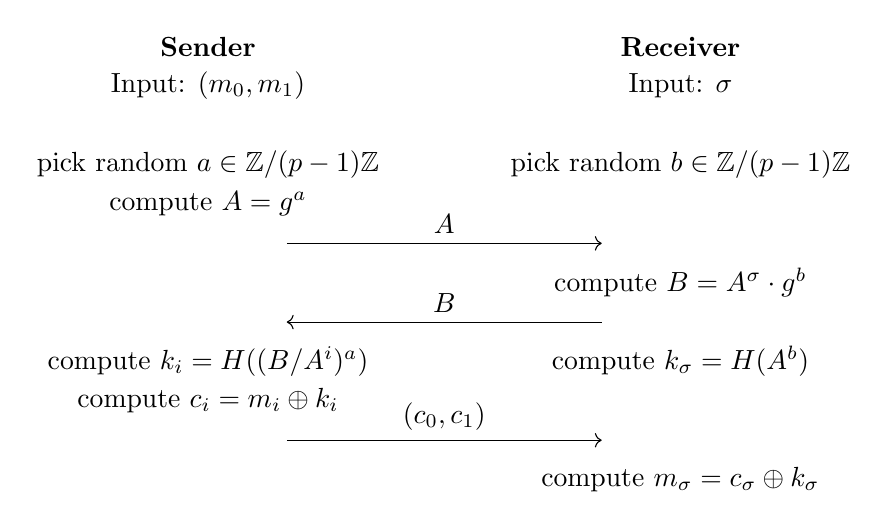
\begin{tikzpicture}
            \node at (0,0) {\bf Sender};
            \node at (6,0) {\bf Receiver};
            \node at (0,-0.5) {Input: $(m_0,m_1)$};
            \node at (6,-0.5) {Input: $\sigma$};
            \node at (0,-1.5) {pick random $a\in\Zn{(p-1)}$};
            \node at (0,-2) {compute $A=g^a$};
            \node at (6,-1.5) {pick random $b\in\Zn{(p-1)}$};          
            \draw[->] (1,-2.5) to node[auto] {$A$} (5,-2.5);
            \node at (6,-3) {compute $B=A^\sigma\cdot g^b$};
            \draw[->] (5,-3.5) to node[above] {$B$} (1,-3.5);
            \node at (0,-4) {compute $k_i=H((B/A^i)^a)$};
            \node at (6,-4) {compute $k_\sigma=H(A^b)$};
            \node at (0,-4.5) {compute $c_i=m_i\oplus k_i$};
            \draw[->] (1,-5) to node[above] {$(c_0,c_1)$} (5,-5);
            \node at (6,-5.5) {compute $m_\sigma=c_\sigma\oplus k_\sigma$};
            \end{tikzpicture}
        \end{center}
    \end{frame}

    \begin{frame}
        \frametitle{The main issue of the simplest OT}
        
        \begin{block}{How to extract input?}
            In case of a corrupted receiver, the simulator extracts the choice bit from the query $A^b$ for the decryption key by the receiver: from this, the simulator knows $g^{ab}$ and may get $\sigma$ from $B^a=g^{a^2\sigma}g^{ab}$.
            
            Upon obtaining $\sigma$, the simulator can query the functionality and compute a ciphertext decrypting to the right $m_\sigma$.
        \end{block}
    
        \pause
        \begin{alertblock}{The issue}
            What if the corrupted receiver computes the key \emph{after} having received the ciphertexts?
            
            The simulator has to send a choice bit to the trusted party before sending the ciphertexts; however it can't know the correct $\sigma$, and the environment can distinguish.
        \end{alertblock}
    \end{frame}
   
    \begin{frame}
        \frametitle{The Algebraic Group Model}
        
        \begin{exampleblock}{The solution}
            We extract at a different point of the execution!
            
            We need additional information, though.
        \end{exampleblock}
    
        \begin{block}{Algebraic behaviour}
            In AGM we impose that whenever the adversary ouptuts an $h\in G$, it also ouputs $h=\prod g_i^{x_i}$, where $g_i$ are group elements that it has already seen.
        \end{block}
    
        \begin{block}{How it helps}
            When the adversary outputs the value $B$, it must give an explanation in terms of $A$ and the public generator $g$. In particular, the simulator learns $B=A^xg^y$; if $x\in\bin$ we have extracted $\sigma$, otherwise we will use random messages.
        \end{block}
    \end{frame}

    \begin{frame}
        \frametitle{The security of CO in the AGM}
        
        \begin{block}{The result}
            In their paper, Abdalla et al. prove UC-security against adaptive malicious adversaries of the Chou and Orlandi protocol in the AGM.
        \end{block}
    
        \begin{block}{The proof}
            Using the equation $B=A^xg^y$, the authors construct a simulation if $x\in\bin$, querying the functionality for $m_x$.
            
            The environment should only be able to check if $m_\sigma$ is the correct one, but should not be able to decrypt the other message; this means not knowing the key $k_{1-\sigma}$, i.e. it shouldn't know the group element $g^{ab}g^{\pm a^2}$.
            
            The authors argue that indeed the adversary cannot know the other key, since from its group representation and the representation of $B$, the adversary could have computed a discrete logarithm.
        \end{block}
    \end{frame}

    
    \section{The Explicit Isogeny model}
        
    \begin{frame}
        \frametitle{Our solution}
        
        \begin{block}{The plan}
            \begin{itemize}
                \item Take a semi-honest two round OT protocol based on isogenies.
                \item Propose a new model, similar to AGM, called \emph{Explicit Isogenies}.
                \item Prove that the protocol is UC-secure against malicious adversaries in the EI model.
                \item {\color{gray}Prove that the EI model is equivalent to plain model of computation.}
                \item Get a post-quantum two-rounds OT protocol that is secure against malicious adversaries.
            \end{itemize}
        \end{block}
    \end{frame}

    \begin{frame}
        \frametitle{The protocol}
        
        \begin{center}
                %\resizebox{0.7\textwidth}{!}{
                \myproc[codesize=\scriptsize]{Protocol $\Pi_{tw}$}{
                    \textbf{Sender} \> \> \textbf{Receiver} \\
                    \text{Input: }(m_0, m_1) \> \> \text{Input: }\sigma \\
                    s \sample Cl(\Oc) \> \> r \sample Cl(\Oc) \\
                    A = s\star E \> \>  C = r\star E \\
                    \> \> \text{if } \sigma=1: C=C^t \\
                    \> \sendmessageleft*{C} \> \\
                    k_0 = H(s\star C) \> \>\\
                    k_1 = H(s\star C^t) \> \>\\
                    c_i = \enc_{k_i}(m_i) \> \> \\
                    \> \sendmessageright*{A, (c_0, c_1)} \> \\
                    \> \> k_\sigma = H(r\star A) \\
                    \> \> m_\sigma= \dec_{k_\sigma}(c_\sigma) \\
                }
            %}
        \end{center}

    \end{frame}

    \begin{frame}
        \frametitle{The EI model}
        
        \begin{definition}
            We say that a Turing machine $\adv$ \emph{uses CM-explicit isogenies} if whenever it outputs a supersingular elliptic curve $E/\F_p$, it also outputs a smooth norm ideal $\mathfrak a\in Cl(\Oc)$ such that $E=\mathfrak a\star E_1$, where $E_1$ is a curve that it has already seen, or its twist.
        \end{definition}
    
    
        \pause
        \begin{theorem}
            The protocol $\Pi_{tw}$ CMEI-realizes the functionality $\Fun_{OT}$ against malicious adversaries.
        \end{theorem}
    
        \begin{proof}
            We follow the proof of the simplest OT in AGM: we extract from the public key explanation. If the adversary can know ``forbidden" keys, a CSIDH vectorization problem can be solved. 
        \end{proof}
    \end{frame}

    \begin{frame}
        \frametitle{The missing step}
        
        \begin{block}{Sampling problem}
            \includegraphics[width=\linewidth]{images/DeFeo_twitter}
        \end{block}
    
        \begin{block}{The consequences}
            If sampling is indeed hard, and people start using it as an assumption, EI model should impose no true additional restrictions.
            
            Caveat: we need to be able to convert isogeny walks into smooth ideals; another open problem. Or maybe not?
        \end{block}
   
    \end{frame}

    \begin{frame}
        \frametitle{Conclusions}
        
        \begin{block}{Results}
            \begin{itemize}
                \item New model for analyzing the security of isogeny-based MPC protocols.
                \item Improved security for a two-round OT protocol.
                \item If sampling problem is hard, the EI model is equivalent to UC.
            \end{itemize}
        \end{block}
    
        \begin{block}{Future work}
            \begin{itemize}
                \item Study other isogeny-based protocols, trying to make them more efficient.
                \item Implement and benchmark different versions of the protocols.
                \item Investigate the sampling problem and its hardness.
                \item Investigate the possible equivalence of isogeny walks and the CM action.
            \end{itemize}
        \end{block}
    \end{frame}

    \begin{frame}
    \begin{center}
        \huge Thanks for your attention!
    \end{center}
    \end{frame}

\end{document}